\documentclass{article}
\usepackage[utf8]{inputenc}
\usepackage{amsmath, amsthm, amssymb}
\usepackage{graphicx} % fugures
\usepackage{wrapfig} %figuras con texto al lado
\usepackage{float} 
\usepackage{siunitx}
\usepackage{mathrsfs}
\usepackage{parskip} % remove the indent 
\usepackage{empheq} % close equations with align in a box / for one eq. to use only \boxed

\title{Cosmología. Marco Teórico}
\author{Margionet Díaz}
\date{December 2018}

\begin{document}

\maketitle

\section{Principio Cosmológico}

La isotropía de la Radiación del Fondo Cósmico de Microondas (CMB) nos dice que a primera aproximación el Universo es isotrópico y homogéneo actualmente. Esto último fue asumido en 1917 por Einstein en su modelo estático, que sería el primer modelo del Universo autoconsistente (Einstein, 1917). También, los modelos de Friedman tiempo después se convertirían en los modelos estándar para las dinámicas a gran escala del Universo y eran basados en soluciones de expansión de las ecuaciones de Einstein siguiendo las pistas de de Sitter y Lanczos.



Con respecto a las coordenadas del espacio y tiempo utilizadas, en 1923 Hermann Weyl introdujo su ``Postulado de Weyl'' (Weyl, 1923) que establecía la noción de geodésicas divergentes, las cuales representan las líneas de mundo de galaxias, que no se intersectan excepto en un punto singular del pasado finito o infinito. Según esto, existe sola una geodésica pasando a través de cada punto en el espacio-tiempo, excepto en el origen.  De aquí es posible asignar un observador a cada línea de mundo. A esto se le conoce como {\textit{Observadores fundamentales}} donde cada uno de ellos lleva un reloj estándar y el tiempo medido en ese reloj desde el punto singular se llama {\textit{tiempo cósmico}}.

En 1935 Robertson y Walker (Robertson, 1935; Walker, 1936) derivaron la métrica del espacio-tiempo para todos los modelos de Universos isotrópicos, homogéneos y en expansión uniforme la cual era independiente de la suposición de que las dinámicas a gran escala eran descritas por la Teoría de la Relativdad General, i.e., no importaba cual fuera la física de la expansión,  la forma de la métrica era la de Robertson - Walker, esto partiendo del supuesto de isotropía y homogeneidad del Universo. 

Otra consideración para construir un modelo cosmológico es el conocido {\bf{principio cosmológico}} de donde podemos afirmar que: ``no estamos ubicados en ningún lugar especial en el Universo'', no hay preferencia, por lo que cualquier observador fundamental ubicado en cualquier lugar del Universo pero en la misma época cósmica observa las mismas características a grande escala que nosotros, i.e., la misma expansión de Hubble de la distribución de galaxias, la misma radiación del CMB isotrópica, la misma estructura esponjosa a gran escala de la distribución de galaxias y vacíos (red cósmica), y así sucesivamente. 
En un sistema de galaxias que se expanden, cada observador en cada galaxia individual observa el mismo flujo de Hubble en la misma época, así, todos tienen derecho a creer que son el centro de un Universo en expansión. 

En cuanto a la geometría, a finales del siglo XVIII se estaban considerando los espacios no euclidianos. Los padres de la geomtría no euclidiana Nikolai Ivanovich Lobachevsky en Rusia y János Bolyai en Transilvania (Lobachevsky, 1829; Bolyai, 1830). Lobachevsky resolvió el problema de la existencia de geometrías no euclidianas, así la misma se puso sobre una base teórica sólida por los estudios de Bernhard Riemann. 

 \begin{wrapfigure}{r}{0.4\linewidth}          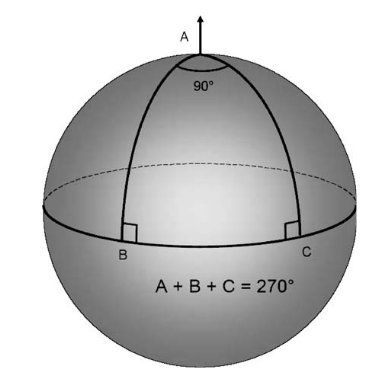
\includegraphics[width=0.5\textwidth]{superficie_esferica_pp152.png}
    \caption{\footnotesize{Suma de los ángulos de un triángulo en la superficie de una esfera}}
    \end{wrapfigure}
    
A través de la geometría riemanniana, Einstein fue capaz de combinar la relatividad especial con la teoría de la gravedad y el cálculo tensorial, lo que fue un logro monumental de la época. Fue así como Einstein se dio cuenta que tenía las herramientas necesarias con las que podría construir modelos totalmente coherentes del Universo, donde su propuesta era un Universo estático, cerrado y con geometría esférica isotrópica. Por otro lado, los modelos de Friedman eran también modelos isotrópicos pero con soluciones de expansión que incluían geometrías que eran tanto esféricas como hiperbólicas (Friedman, 1922, 1924). 

En la figura 1 se tiene el caso más simple de la geometría curvada en 2 dimensiones, la superficie de una esfera: un triángulo con dos líneas (con $90^{\circ}$ entre ellas) que parten del polo norte y llegan hasta el ecuador, y una tercera línea que se dibuja sobre el ecuador. Estas líneas son la distancia más corta entre entre las tres esquinas del triángulo. En geometría curva son geodésicas. 

De fig. 1, si el radio de una esfera es $R_c$, el área superficial del triángulo ABC es $A= \theta R_c$ y variando el ángulo se obtiene para $\theta = 90^{\circ} \rightarrow{A = \pi R_c^2/2}$ y la suma de los ángulos del triángulo es $270º$ y si $\theta=0º$ entonces el área es cero y la suma de los ángulos $180º$. Así, la diferencia de la suma de los ángulos de $180º$ es proporcional al área del triángulo:
$$(\text{suma de los ángulos del triángulo} - 180º \propto \text{área del triángulo},$$
la cual es una propiedad general de los espacios curvos isotrópicos. 

   \vspace{0.5cm}

\subsection{La métrica espacio-tiempo para espacios isotrópicos curvos}

\begin{equation}
  dl^2 = dx^2 + dy^2 + dz^2,  
\end{equation}
Representa la distancia entre dos puntos separados por $dx, dy, dz$ en un espacio plano. 

Siendo el caso más simple de un espacio curvo bidimensional isotrópico la superficie de una esfera, es conveniente utilizar un sistema coordenado polar para describir posiciones en la superficie (ver figura 1) que para el caso, las coordenadas ortogonales son $\theta$ y $\phi$ y el aumento de la distancia $dl$ entre dos puntos en dicha superficie es:

\begin{equation}
    dl^2 = R_c^2 d\theta^2 + R_c^2 \sin^2 \theta d\phi^2,
\end{equation}

    donde $R_c$ es el radio de curvatura de la superficie del espacio bidimensional, para el caso, el radio de la esfera. (2) es la {\textit{métrica de la superficie bidimensional}} y puede generalizarse como:
    
    \begin{equation}
        dl^2 = g_{\mu \nu} dx^{\mu} dx^{\nu}, 
    \end{equation}
    
    siendo el {\textit{tensor métrico}} el contenedor de toda la información acerca de la geometría intrínseca del espacio. Otros sistemas de coordenadas pueden definir las coordenadas de un punto en cualquier superficie bidimensional. Para un plano euclidiano: 

\begin{equation}
    dl^2 = dx^2 +  dy^2,
\end{equation}

en polares

\begin{equation}
    dl^2 = dr^2 + r^2 d\phi^2.
\end{equation}

Con el tensor métrico $g_{\mu \nu}$ es posible determinar la curvatura intrínseca del espacio, y esto fue probado por Gauss. Para tensores que pueden ser reducidos a la forma diagonal (ecs. 2, 4, 5) la curvatura intrínseca viene dada por:


    \begin{align*}
        \kappa & = \frac{1}{2 g_{11} g_{22}} \left\{ - \frac{\partial^2g_{11} }{\partial x_2^2} - \frac{\partial^2g_{22} }{\partial x_1^2} + \frac{1}{2 g_{11}} \left[ \frac{\partial g_{11} }{\partial x_1} \frac{\partial g_{22} }{\partial x_1} +   \left( \frac{\partial g_{11} }{\partial x_2} \right)^2 \right] 
        + \frac{1}{2 g_{22}} \left[ \frac{\partial g_{11} }{\partial x_2} \frac{\partial g_{22} }{\partial x_2} + \left( \frac{\partial g_{22} }{\partial x_1} \right)^2 \right] \right\} 
    \end{align*}

$\kappa$ se conoce como la {\textit{curvatura gaussiana}} del bi-espacio. La extención a tres espacios isotrópicos es sencilla si mantenemos que cualquier sección bidimensional a través de un espacio tridimensional isotrópico debe ser un bi-espacio isotrópico y ya el tensor métrico par este caso es conocido. 

Fue mencionado que para un bi-espacio isotrópico, las coordenadas adecuadas son las polares esféricas. De la fig. 2, la distancia alrededor del arco de un gran círculo desde el punto $O$ hasta $P$ es $R_c \theta$, por lo que la métrica se escribe:

    \begin{equation}
        dl^2 = d\varrho^2 + R_c^2 \sin^2\left(\frac{\varrho}{R_c} \right) d\phi^2,
    \end{equation}

donde $\varrho$ es la distancia más corta entre $0-P$  en la superficie de una esfera ya que es parte de un gran  círculo. De esta manera, estamos hablando de una {\textit{distancia geodésica}} en el espacio curvo isotrópico. Recordemos que en espacios curvos las geodésicas juegan el rol de las líneas rectas.

    \begin{wrapfigure}{r}{0.5\linewidth}               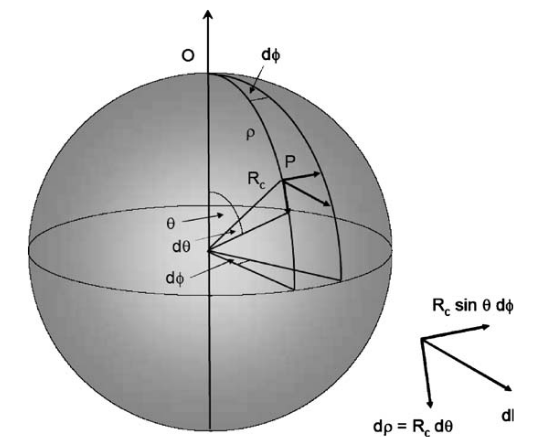
\includegraphics[width=0.5\textwidth]{superficie_esferica_pp156_angulos.png}
        \caption{\footnotesize{$\varrho$ es la distancia radial alrededor de la esfera desde el polo y el ángulo $\phi$ mide los desplazamientos angulares en el polo.}}
    \end{wrapfigure}

Ahora, (6) puede ser reescrita como: 

    \begin{equation}
        x = R_c \sin \left(\frac{\varrho}{R_c} \right).
    \end{equation}
    
    Hallando $dx^2$ con $$d\varrho^2 = \frac{dx^2}{1-\kappa x^2},$$
    la métrica puede ser escrita como: 
    
    \begin{equation}
        dl^2 = \frac{dx^2}{1-\kappa x^2} + x^2d\phi^2.
    \end{equation}
    
    \vspace{0.6cm}
    Recordando que $\kappa = 1/R_c$, tres casos deben ser considerados: 
    
    \begin{equation*}
     \label{eq:aqui-le-mostramos-como-hacerle-la-llave-grande}
     \kappa  = \left\{
	       \begin{array}{ll}
		 > 0      & {\text{espacio esférico}},, \\
		 = 0 & R_c \rightarrow{\infty}, \hspace{0.4cm}  {\text{espacio plano}}, \\
		 < 0     & {\text{espacio hiperbólico}}.
	       \end{array}
	     \right.
   \end{equation*}
    
    \vspace{0.4cm}
    
Para $\kappa = 0$ se recupera el espacio euclidiano.

Para el incremento espacial en un espacio tridimensional curvo recordemos que cualquier sección bidimensional a través de un tri-espacio isotrópico debe ser un espacio isotrópico de dos dimensiones donde la métrica puede ser ec. (6) o (8). En coordenadas polares esféricas, el desplazamiento angular general perpendicular a la dirección radial es 
\begin{equation}
    d\phi^2 = d\theta^2 +  \sin^2 \theta d\phi^2.
\end{equation}
 (con $\theta$ y $\phi$ diferentes a los usados en la figura 2). De esta manera, se puede escribir el incremento espacial (de 6 y 8) 


\begin{align}
        dl^2 & = d\varrho^2 + R_c^2 \sin^2\left(\frac{\varrho}{R_c} \right) [d\theta^2 +  \sin^2 \theta d\phi^2], \\
        dl^2 &  =  \frac{dx^2}{1-\kappa x^2} + x^2[d\theta^2 +  \sin^2 \theta d\phi^2].
\end{align}

De esta manera, la {\textit{métrica de Minkowski}} para un tri-espacio isotrópico viene escrita como: 

\begin{equation}
    ds^2 = dt^2 - \frac{1}{c^2} dl^2,
\end{equation}

con $dl$ el de las expresiones (10) u (11). Aunque $x$ y $\varrho$ son medidas de distancias equivalente, su significado físico es bastante distinto. A continuación, podemos derivar la métrica de Robertson -  Walker. 


\subsection{Métrica de Robertson - Walker}

Queremos aplicar la métrica de Minkowski, ec. 12, a modelos de mundo homogéneos, isotrópicos. Para eso, debemos recurrir a:

    \begin{enumerate}
        \item Principio cosmológico: A primera aproximación, el Universo es isotrópico y homogéneo en la época actual.
        \item Observadores fundamentales: quienes se mueven de modo tal que el Universo siempre parece isotrópico para ellos. 
        \item Tiempo cósmico: cada uno de estos observadores lleva un reloj y el tiempo propio medido por ese reloj es lo que se conoce como {\textit{tiempo cósmico}}.
    \end{enumerate}
    
Recordemos que según el postulado de Weyl, las geodésicas de todos los observadores se reunen en un punto en el pasado y el tiempo cósmico puede ser medido desde esa época de referencia. 

Ahora bien, considerando las ecs. 10 y 12, podemos escribir la métrica como:

    \begin{equation}
        ds^2 = dt^2 - \frac{1}{c^2}( d\varrho^2 + R_c^2 \sin^2\left(\frac{\varrho}{R_c} \right) (d\theta^2 +  \sin^2 \theta d\phi^2)],
    \end{equation}

siendo $t$ el tiempo cósmico y $d\varrho$ un incremento de la distancia propia en la dirección radial. 

Para un Universo en expansión, esta métrica presenta problemas. Ya que la luz viaja una velocidad finita, observamos todos los objetos astronómicos a lo largo de un cono de luz anterior centrado en la Tierra en la época actua $t_0$ (ver figura 3). Así, cuando observamos objetos distantes, no los observamos en la época actual sino en un tiempo anterior $t_1$, cuando el Universo todavía era homogéneo e isotrópico, pero las distancias entre los fundamentales eran menores y la curvatura espacio diferente. Significa entonces que la métrica 13 solo puede ser aplicada a un espacio curvo, isotrópico definido en una única época. 

\begin{wrapfigure}{r}{0.5\linewidth}               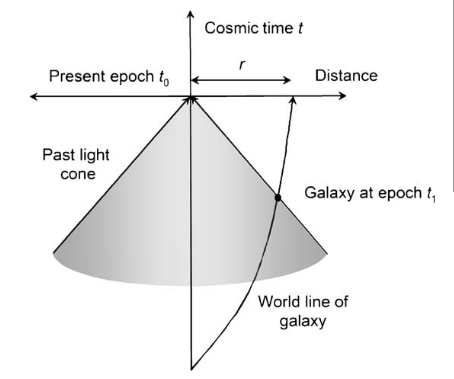
\includegraphics[width=0.65\textwidth]{cono_luz_pp159.png}
        \caption{\footnotesize{Diagrama de espacio-tiempo que ilustra la definición de la distancia de la coordenada radial comovil.}}
    \end{wrapfigure}
    
    
Para medir una distancia propia adecuada que pueda ser incluida en (13)  se pueden alinear un conjunto de observadores fundamentales que estén entre la Tierra y la galaxia. Cada uno de estos observadores va a medir la distancia $d \varrho$ a su próximo observador en un tiempo cósmico particular. Al sumar todos estos $d \varrho$ se puede obtener una distancia adecuada que es medida en una sola época y con la que sería posible incluir en la métrica (13). Lo que nosotros observamos son galaxias distantes en una época pasada, i.e., cómo eran en una época anterior, y no se sabe cómo proyectar sus posiciones relativas a nosotros en la época actual hasta que conozcamos la cinemática del Universo en expansión. Es por esto que la distancia depende de la elección del modelo cosmológico que se considere. 

En una expansión uniforme la distancia entre dos observadores fundamentales, $i,j$ en dos épocas $t_1$ y $t_2$ cambia de manera que 

    \begin{align}
        \frac{\varrho_i(t_1)}{\varrho_j(t_1)} & = \frac{\varrho_i(t_2)}{\varrho_j(t_2)} = {\text{constante}} \notag \\
        \frac{\varrho_i(t_1)}{\varrho_i(t_2)} & = \frac{\varrho_j(t_2)}{\varrho_j(t_2)} = ... =  {\text{constante}} = \frac{a(t_1)}{a(t_2)}.
    \end{align}


En modelos isotrópicos, $a(t)$ representa una función universal conocida como {\bf{factor de escala}}, la cual explica cómo la distancia entre cualquiera de los dos observadores fundamentales cambia con el tiempo cósmico $t$. 
Si tomamos $a(t) = 1$ para la época presente, $t_0$, y renombramos el valor de $\varrho$ en el presente como $r$, (14) se escribe como

    \begin{equation}
        \varrho (t) = a(t)r,
    \end{equation}

donde $r$ lleva la etiqueta de distancia, la cual está unida a una galaxia u observador fundamental durante todo el tiempo y recibe el nombre de {\bf{coordenada de distancia radial comóvil}}. La variación en la distancia propia en el Universo en expasión es $a(t)$. Las distancias propias perpendicular a la línea de visión también pueden cambiar por un factor $a$ entre $t_0$ y $t$, a causa de la isotropía de y homogeniedad del modelo, 

\begin{equation}
    \frac{\Delta l(t)}{\Delta l(t_0)} = a(t).
\end{equation}

De la métrica (13) 

    \begin{align}
        a(t) & = \frac{R_c(t) \sin[\varrho/R_c(t)] d \theta}{R_c(t_0) \sin[r/R_c(t_0)] d \theta}, \\
    \frac{R_c(t)}{a(t)} \sin \left[\frac{a(t)r}{R_c(t)} \right] & = R_c(t_0) \sin \left[\frac{r}        {R_c(t_0)} \right],
    \end{align}

válido siempre que 
    \begin{equation}
        R_c (t) = a(t) R_c (t_0),
    \end{equation} 

de aquí que, para conservar la isotropia y homegeindad, {\bf{la curvatura del espacio cambia a medida que el Universo se expande}} como $k = R_c^{-2} \propto a^{-2}$. 

Si ahora el radio de curvatura de la geometría del espacio $R_c$ en la época presente lo etiquetamos como R'
    \begin{equation}
        R_c (t) = a(t) R'.
    \end{equation}

Sustituyendo (15) y (19) en (13):

    \begin{equation}
        ds^2 = dt^2 - \frac{a^2(t)}{c^2} [dr^2 + R'^2 \sin^2(r/R')(d \theta^2 + \sin^2 \theta d\phi^2)],
    \end{equation}

obtenemos la {\bf{métrica de Robertson - Walker}}, la cual contiene dos incognitas: 

    \begin{enumerate}
        \item La función desconocida pero etiquetada como el factor de escala $a(t)$, que describe la dinámica del Universo,
        \item La constante, también desconocida, $R'$, la cual describe la curvatura espacial del Universo en la época presente. 
    \end{enumerate} 

También, si se usa la {\bf{distancia de diámetro angular comóvil}}: $r_1 = R' \sin(r/R')$, la métrica puede ser escrita como:

    \begin{equation}
        ds^2 = dt^2 - \frac{a^2(t)}{c^2} \left[ \frac{dr_1^2}{1 - \kappa r_1^2} + r_1^2 (d\theta^2 + \sin^2 \theta d\phi^2) \right],
    \end{equation}

    siendo ahora $\kappa = 1/R'^2$. Además, por un reescalamiento adecuado de la coordenada $r_1$: $\kappa r_1^2=r_2^2$, la métrica se escribe:

    \begin{equation}
        ds^2 = dt^2 - \frac{R_1^2(t)}{c^2} \left[ \frac{dr_2^2}{1 - \kappa r_2^2} + r_2^2 (d\theta^2 + \sin^2 \theta d\phi^2) \right],
    \end{equation}

donde $\kappa = +1, 0 -1$ para universos con geometría esférica, plana o hiperbólica. En este reescalamiento $R_1(t)= R_c(t_0) a= R'a$ por lo que $R_1(t)$ en la época presente es $R'$ más bien que la unidad. 
Las métricas (19), (20) y (21) pueden definirnos el intervalo invariante $ds^2$ entre eventos en cualquier época o lugar en el Universo en expansión. 

Finalmente, vamos a repasar algunos aspectos importantes:

    \begin{enumerate}

        \item El {\bf{tiempo cósmico $t$}} es el tiempo medido por un reloj llevado por el observador fundamental,
        \item {\bf{$r$ es la coordenada de distancia radial comovil}} que está fija a una galaxia para siempre y que es la distancia propia que tendría la galaxia si sus líneas de mundo fueran proyectadas hacia adelante a la época $t_0$ y sus distancias medidas en ese tiempo. 
        \item $a(t)dr$ es el {\bf{elemento de distancia propia (geodésica) en la dirección radial en la época}} $t$. 
        \item $a(t) [R'\sin(r/R')] d\theta = a(t) r_1 d\theta$ es el {\bf{elemento de distancia propia perpendicular a la dirección radial subtendida por el ángulo}} $d\theta$ en el origen. 
        \item $a(t) [R'\sin(r/R')] \sin \theta d\phi = a(t) r_1 \sin \theta d\phi$ es el {\bf{elemento de distancia propia en la dirección}} $\phi$.
        
        No sabemos nada acerca de la física que gobierna la tasa de expansión de Universo; sin embargo, $a(t)$ absorbe este fenómeno todavía desconocido.  
        
    \end{enumerate} 



\section{Observaciones en Cosmología}

\subsection{Corrimiento al Rojo Cosmológico}

Cuando hablamos del corrimiento al rojo cosmológico, nos referimos al desplazamiento de las líneas espectrales hacia longitudes de onda más grandes asociadas a la expansión isotrópica del sistema de galaxias. Así, el corrimiento al rojo $z$ es definido como

\begin{equation}
    z = \frac{\lambda_0 - \lambda_e}{\lambda_e},
\end{equation}

siendo $\lambda_0$ la longitud de onda observada y $\lambda_e$ la longitud de onda de la línea emitida.  



Si $z$ fuera interpretada como una velocidad de recesión $v$ de una galaxia, $z$ y $v$ serían relacionadas por el desplzamiento Doppler Newtoniano

    \begin{equation}
        v= cz,
    \end{equation}

que fue utilizada por Hubble para derivar la relación velocidad-distancia, $v=H_0 r$. 

En cosmología, el corrimiento al rojo tiene un significado más profundo. Por ejemplo, si consideramos un paquete de ondas de frecuencia $\nu_1$ emitido entre los tiempos cósmicos $t_1$ y $t_1 +  \Delta t_1$ de una galaxia distante, y es recibido por un observador en la época presente $t_0$ y $t_0 + \Delta t_0$, la señal se propaga a lo largo de {\bf{conos nulos}}, $ds^2=0$, y si además $d\theta = d\phi = 0$, la métrica (19) puede escribir como:

    \begin{equation}
        dt = - \frac{a(t)}{c} dr \hspace{0.4cm} \frac{c dt}{a(t)} = -dr,
    \end{equation} 

con $a(t) dr$ el {\bf{intervalo de distancia propia en el tiempo cósmico}} $t$. Para el borde delantero del paquete de ondas 

    \begin{equation}
        \int_{t_1}^{t_0} \frac{cdt}{a(t)} = - \int_r^0{dr}.
    \end{equation}
        
Y el final del paquete de ondas debe viajar la misma distancia en unidades de la coordenada de distancia comovil ya que $r$ es fija a la galaxia para siempre. Así:

    \begin{align} 
        \int_{t_1 + \Delta t_1}^{t_0 + \Delta t_0}{ \frac{cdt}{a(t)}} & = - \int_r^0{dr}, \\
        \int_{t_1}^{t_0}{ \frac{cdt}{a(t)} +  \frac{c \Delta t_0}{a(t_0)} -\frac{c \Delta t_1}{a(t_1) }}   & =  \int_{t_1}^{t_0}{ \frac{cdt}{a(t)}}. 
     \end{align}

 Y ya que $a(t_0) = 1$

    \begin{equation}
        \Delta t_0 = \frac{\Delta t_1}{a(t_1)}.
    \end{equation}


Esta es la expresión para el fenómeno de la {\bf{dilatación del tiempo}}. Galaxias distantes son observadas en algún tiempo cósmico anterior $t_1 < 1$ por lo que se observa que los fenómenos tardan más en nuestro marco de referencia que en el de la fuente. 

( El fenómeno es precisamente lo mismo que la dilatación del tiempo en la relatividad especial, por lo que, por ejemplo, se observa que los muones relativistas, creados en la parte superior de la atmósfera, tienen vidas más largas en el marco del observador en comparación con sus tiempos de vida propios. 
Dilatación del tiempo: La dilatación del tiempo es el fenómeno predicho por la teoría de la relatividad, por el cual un observador observa que el reloj de otro (un reloj físicamente idéntico al suyo) está marcando el tiempo a un ritmo menor que el suyo. Esto se suele interpretar normalmente como que el tiempo se ha ralentizado para el otro reloj, pero eso es cierto solamente en el contexto del sistema de referencia del observador. Localmente, el tiempo siempre está pasando al mismo ritmo. El fenómeno de la dilatación del tiempo se aplica a cualquier proceso que manifieste cambios a través del tiempo y espacio.)


(29) nos da una expresión para el corrimiento al rojo. Si $\Delta t_1 = \nu_1^{-1}$ es el periodo de las ondas emitidas y  $\Delta t_0 = \nu_0^{-1}$ el período observado, para la ec. 29 ahora se escribe como

\begin{equation}
    \nu_0 = \nu_1(t_1) a(t_1),
\end{equation}

y de (23) y usando (30) 

\begin{align}
     z & = \frac{\lambda_0 - \lambda_e}{\lambda_e} = \frac{\lambda_0 }{\lambda_e} - 1 = \frac{\nu_1}{\nu_0}, \\
     z + 1 & = \frac{\nu_1}{\nu_0} = \frac{1}{a(t_1)}, \hspace{0.3cm} \text{finalmente} \\
     a(t_1) & = \frac{1}{z+1}
\end{align}


De aquí que el corrimiento al rojo es una {\bf{medida del factor de escala del Universo cuando la fuente emitió la radiación}}. 
Cuando observamos una galaxia con desplazamiento al rojo $z = 1$, el factor de escala del Universo cuando se emitió la luz fue $a (t) = 0.5$, i.e., las distancias entre observadores fundamentales (o galaxias) eran la mitad de sus valores actuales

(a (t) es una función universal conocida como el factor de escala que describe cómo las distancias relativas entre cualquiera de los dos observadores fundamentales cambian con el tiempo cósmico t.)

De (26) podemos obtener una expresión para la {\bf{coordenada de distancia radial comovil}} $r$:

    \begin{equation}
        r = \int_{t_1}^{t_0}{\frac{c dt }{a (t)}}.
    \end{equation} 

    $r$ {\bf{es una distancia artificial que depende de cómo el Universo se ha expandido entre la emisión y recepción de la radiación}}.

La dilatación del tiempo, expresión 28, está relacionada con las supernovas tipo 1a (SN 1a). La estrecha dispersión en sus magnitudes absolutas que tiene exactamente la misma curva de luz  (la variación en el tiempo en sus luminosidades durante la explosión de la SN) ha hecho que estos objetos sean herramientas útiles en cosmología. Las grandes luminosidades de las SN tipo 1a hace que estas puedas ser observadas a altos corrimiento al rojo. 


Otra prueba de la dilatación del tiempo usando las propiedades de las SN Ia es usar la evolución espectral como un reloj para comparar el tiempo de evolución de SN de alto y bajo redshift. Usando la SN 1997ex, la cual tenía un $z= 0.361$, el tiempo entre el primero y segundo espectro fue de $24.88$ días y entre el primero y tercero de $30.95$ días. La cantidad de envejecimiento en el marco en reposo de la SN debe ser un factor $1/(z+1)$ menor a las edades de $18.28$ y $22.74$ días. La técnica de las edades aplicada a la SN fueron de $16.97 \pm 2.75$ días y $18.01 \pm 3.14$ días, en excelente acuerdo con lo esperado de la dilatación de tiempo cosmológico. 

% FALTAN IMÁGENES 178 PDF. 

\subsection{Ley de Hubble} 

(The distance $\varrho$ is the shortest distance between O and P on the surface of the sphere
since it is part of a great circle and is therefore the geodesic distance between O and
P in the isotropic curved space)
($d \varrho$ is an increment of proper distance in the radial direction.)
(Thus, the distance $\varrho$ measure depends upon the choice of cosmological model.

La ley de Hubble puede escribirse como: 


 \begin{equation}
        \frac{\varrho}{dt} = H\varrho,
    \end{equation}

con $\varrho$ la distancia propia, $\varrho = a(t) r$. Usamos $H$ en vez de $H_0$ porque vamos a considerar la {\bf{``constante de Hubble''}} en cualquier época y no en el presente. Sustituyendo $\varrho = a(t) r$,

    \begin{align}
        r\frac{da(t)}{dt} & = Ha(t)r, \\
        H = \frac{\dot{a}}{a}.
    \end{align}

Si consideramos la constante de Hubble en el tiempo presente, $t= t_0$, $a=1$, entonces 
    \begin{equation}
        H_0 = (\dot{a})_{t_0}.
    \end{equation}

La {\bf{constante de Hubble define la tasa de expansión del Universo en el presente}}. Para cualquier época podemos definir: 

    \begin{equation}
        H(t) = \frac{\dot{a}}{a}.
    \end{equation}

\subsection{Diámetros angular}

En la sección anterior, hemos considerado únicamente la parte radial. Siguiendo con la métrica de Roberton - Walker 

        $$ds^2 = dt^2 - \frac{a^2(t)}{c^2} [dr^2 + R'^2 \sin^2(r/R')(d \theta^2 + \sin^2 \theta d\phi^2)],$$
  
  consideraremos ahora el componente espacial relevante $d\theta$. La longitud propia $d$ de un objeto en el desplazamiento al rojo $z$, correspondiente al factor de escala $a(t)$ viene dado por el incremento de la longitud propia perpendicular a la dirección radial:
  
  \begin{align}
      d & = a(t) R' \sin \left(\frac{r}{R'} \right) \Delta \theta = a(t) D \Delta \theta = \frac{D \Delta \theta}{1+z}, \\
      \Delta \theta & = \frac{d(1+z)}{D}.
  \end{align}

Donde distinguimos que $D = R' \sin(r/R')$. Para pequeños $z$, $z << 1, r <<R'$ la ec. 41 se reduce a la relación euclidiana $d = r \Delta \theta$. Entonces 41 puede ser escrita también como:

    \begin{equation}
        \Delta \theta = \frac{d}{D_A},
    \end{equation}

donde se ha definido una nueva medida conocida como {\bf{distancia de diámetro angular}}

(Llamemos al valor de $ R_c (t_0) $, es decir, el radio de curvatura de la geometría espacial en la época actual, $ R '$, entonces $R_c(t)= a(t) R'$)
($R'$ es una constante desconocida que describe la curvatura espacial del Universo en la época actual.)

Otro cálculo importante es el del {\bf{diámetro angular de un objeto que continúa participando en la expansión}} como es el caso de una perturbación infinitesimal en la expansión del Universo. Un ejemplo es el diámetro angular que estructuras a gran escala presentes en el Universo actual habrían subtendido en una época anterior, e.g., la recombinación, si simplemente se hubiesen expandido con el Universo. Este se usa para calcular tamaños físicos correspondientes a las escalas angulares de las fluctuaciones observadas en la radiación del CMB. Si el tamaño de un objeto es actualmente de $d(t_0)$ y se expandió con el Universo, su tamaño físico en el desplazamiento al rojo fue de

    $$d(t_0) a(t)=  \frac{d(t_0)}{(1+z)}$$,

por lo tanto, ese objeto subtendió un ángulo

    \begin{equation}
        \Delta \theta = \frac{d(t_0)}{D}.
    \end{equation}

\subsection{Intensidades Aparente}

Se tiene una fuente con luminosidad $L(\nu_1), \mathrm{W Hz^{-1}}$ y con un corrimiento al rojo $z$. Esta $L$ es la energía total emitida sobre $4 \pi$ estereorradián por unidad de tiempo por unidad de intervalo de frecuencia. Siendo $\nu_0$ la frecuencia en la época presente $t_0$, queremos calcular la densidad de flujo $S(\nu_0)$ de la fuente en la frecuencia $\nu_0$ en que esta se observa. Específicamente, ¿cuál es la energía recibida por unidad de tiempo, por unidad de área, por unidad de ancho de banda, en unidades de $\mathrm{W m^{-2} Hz^{-1}}$. De ecs. (30) y (33) 
    $$\nu_0 = a(t_1) \nu_1 = \frac{1}{z+1}.$$

Podemos suponer que la fuente emite $N(\nu_1)$ fotones con energía $h \nu_1$, en el ancho de banda $\nu_1, \nu_1 + \Delta \nu_1$ en el intervalo de tiempo propio $\Delta t_1$. De esta manera $L(\nu_1)$ es

    \begin{equation}
        L(\nu_1) = \frac{N(\nu_1) h \nu_1 }{\Delta \nu_1 \Delta t_1}.
    \end{equation}
    
    Imagine que la fuente, en un tiempo $t_1$, es el centro de una ``esfera'' y que los fotones que ha emitido están distribuidos sobre una ``capa'' que rodea a la esfera. Cuando esta capa de fotones llega al observado, en una época $t_0$, cierta cantidad de ellos son interceptados por un telescopio. En $t_0$, los fotones observados tienen frecuencia $\nu_0 = a(t_1) \nu_1$, de ec. (29), un intervalo de tiempo propio $ \Delta t_0 = \Delta t_1/a(t_1)$ y en el ancho de banda $ \Delta \nu_0 = a(t_1) \nu_1$.

    Para conocer cuántos fotones están sobre esta ``capa'' que rodea la esfera entre la época $t_1$ y $t_0$ es necesario relacionar el diámetro del telescopio $\Delta l$  al diámetro angular $\Delta \theta$ (POR QUÉ USAR Delta y no d?) que subtiende en la fuente en la época $t_1$. De ec. (42), si consideramos que para un tiempo presente, $t_0$, $a(t_0) = 1$
    
    \begin{equation}
        \Delta l = D \Delta \theta,
    \end{equation}
    
    siendo $\Delta \theta$ el ángulo medido por un observador fundamental, el cual se encuentra en la fuente. 
    


    Si ahora introducimos la noción de ángulo sólido $d\Omega$, podemos considerar cómo los fotones que la fuente ha emitido se extienden sobre $d \Omega$, como se observa desde la fuente en la geometría curva. Si se supone que el Universo no se expande, el área superficial sobre la cual se observan los fotones en un tiempo $t$ después de su emisión se escribe como: 

    \begin{equation}
        dA = R_c^2 \sin^2 \frac{x}{R_c} d\Omega,
    \end{equation}

    siendo $x = ct$. Por otro lado, si el Universo se expande, el radio de curvatura $R_c$ cambia como el Universo lo haga, y en lugar de $x/R_c$, tendríamos 

    \begin{equation}
        \frac{1}{R'} \int_{t_1}^{t_0}{\frac{c dt}{a}} =     \frac{r}{R'},
    \end{equation}


    con $r$ la coordenada de distancial radial comóvil. Sustituyendo (48) en (47)

    \begin{equation}
        dA = R'^2 \sin^2 \frac{r}{R'} d\Omega.
    \end{equation} 

    Entonces el diámetro del telescopio como lo vemos desde la fuente es $\Delta l = D \Delta \theta$. Recordemos que las distancia comóviles toman en cuanta la expansión del Universo, a diferencia de las distancias propias. Por lo tanto, el área superficial del telescpio es $\pi \Delta l^2 / 4$ y el ángulo sólido subtendido por esta área superficial en la fuente es $d \Omega = \pi \Delta \theta^2/4$. El número de fotones incidentes sobre el telescopio en un tiempo $\Delta t_0$ es 
    
    \begin{equation}
        N (\nu_1) \frac{\Delta \Omega}{4 \pi},
    \end{equation}

    POR QUE DIVIDIDO ENTRE 4? 
    
    donde ahora ellos son observados con frecuencia $\nu_0$. De esta manera, podemos conocer la expresión para la densidad de flujo de la fuente, i.e., la cantidad de energía recibida por unidad de tiempo, por unidad de área, por unidad de ncho de banda. Esto es
    
    \begin{equation}
        S(\nu_0) = \frac{N (\nu_1) h \nu_0 \Delta \Omega} {4\pi \Delta t_0 \Delta \nu_0 (\pi/4)\Delta l^2 }.
    \end{equation}

    Haciendo uso de las ecs. 30 y 31, además de las relaciones de la luminosidad, 54, y el diámetro del telescopio, 46, podemos expresar 51 como: 
    
    \begin{align}
        S( \nu_0) & = \frac{[N(\nu_1) h \nu_1 (t_1) a(t_1)] (\pi \Delta \theta^2/4)}{4 \pi [\Delta t_1/a(t_1)] [\nu_1 a(t_1)] (\pi/4)(D^2 \Delta \theta^2)}, \\ 
        \\
        S(\nu_0) & = \frac{L(\nu_1) a(t_1)}{4\pi D^2} =\frac{L(\nu_1)}{4\pi D^2(1+z)}.
    \end{align}

    (54) es la mejor expresión para relacionar la intensidad observada $S(\nu_0)$ a la luminosidad intrínseca de la fuente $L(\nu_1)$. 
    
    Para luminosidades y densidades de flujo {\bf{bolométricas}} se considera entonces la energía total emitida en un ancho de banda finito $\Delta \nu_1$ y que es recibida en el ancho de banda $\Delta \nu_0$. Se tiene
    
    \begin{align}
        L_{bol}= L (\nu_1) \nu_1 & = 4 \pi D^2 S(\nu_0)(1+z) \times \Delta \nu_0 (1+z), \\
        & = 4 \pi D^2 (1+z)^2 S_{bol},
    \end{align}

    POR QUÉ EL FACTOR (1+Z)? 

    de donde se desprende que 
    
    \begin{align}
        S_{bol} & = S(\nu_0) \nu_0, \\
        S_{bol}  & = \frac{L_{bol}}{4 \pi D^2 (1+z)^2} =  \frac{L_{bol}}{4 \pi D_L^2}.
    \end{align}
    
    Note la nueva cantidad $D_L =  D (1+z) $, la cual es conocida como la {\bf{distancia de luminosidad }} de la fuente. Esta cantidad $D_L$ que relaciona a $L_{bol}$ con $S_{bol}$ hace que la misma luzca como una ley del  del cuadrado inverso. 
    
    Es posible medir la densidad de flujo bolométrica en la presente época, $t_0$, si integramos la luminosidad bolométrica en cualquier ancho de banda adecuado siempre que se utilice el $z$  correspondiente. Así, 
    
    \begin{equation}
        \sum_{\nu_0} S(\nu_0) \Delta \nu_0 = \frac{ \sum_{\nu_1} L(\nu_1) \Delta \nu_1 }{4 \pi D^2 (1+z)^2} =   \frac{\sum_{\nu_1} L(\nu_1) \Delta \nu_1}{4 \pi D_L^2}
    \end{equation}
    
    Si se conoce el espectro de la fuente $L(\nu)$, la relación (58) puede escribirse en términos de la luminosidad de la fuente en la frecuencia observada $\nu_0$. Esto es:
    
    \begin{equation}
        S(\nu_0) = \frac{L(\nu_0)}{4\pi D_L^2} \left[ \frac{L(\nu_1)}{L(\nu_0)}(1+z) \right]. 
    \end{equation}
    
    El término entre corchetes es lo que se conoce como {\bf{Corrección-$K$}} que es utilizada para ``corregir'' las magnitudes aparetes de galaxias distantes por los efectos de desplazamiento al rojo de sus espectros cuando las observaciones son hechas a través de filtros estándar con una frecuencia de observación fija media $\nu_0$ (Sandage, 1961b).Así, la relación (60) puede escribirse en función de la magnitud absoluta, 
    
    $$M = cte - 2,5 \log_{10} L(\nu_0),$$ 
    y la aparente, 
    
    $$m = cte - 2,5 \log_{10} S(\nu_0),$$ 
    
    encontrándose que
    
    \begin{align}
        M & = m - 5 \log_{10} (D_L) - K(z) - 2.5 \log_{10} (4\pi), \hspace{0.3cm} \text{donde}, \\
        K & = -2.5 \log_{10} \left[ \frac{L(\nu_1)}{L(\nu_0)}(1+z) \right].
    \end{align}
        
    Esta corrección-$K$ es correcta para densidades de flujo y luminosidades \\ 
    {\textit{monocromáticas}}.
    
\subsection{Densidades Numéricas}

    Conocer la cantidad de objetos en un intervalo de corrimiento al rojo $z, z + dz$ es importante. Varias cosas sabemos, que existe una relación uno a uno entre $r$ y $z$, siendo $r$ la {\bf{coordenada de distancia propia radial definida en la presente época}}, resultados que ya fueron dados en sec. 1.1, por lo que ya se conoce el número de objetos en el intervalo de distancia de coordenadas radial cómovil $r, r+dr$. El diagrama de espacio-tiempo (cono de luz, fig. 3) muestra cómo podemos conocer el número de objetos por trabajar en base a los volúmenes comóviles para la presente época. Para este caso, el radio de curvatura de la geometría curva es $R'$, así que el volumen de la concha esférica de grosor $dr$ en la coordenada de distancia comovil $r$ es

    \begin{equation}
        \mathrm{ dV = 4\pi R'^2 \sin^2 (r/R') dr = 4\pi D^2 dr, }
    \end{equation}

    donde identificamos a $R'^2 \sin^2 (r/R') = D^2$. Si $N_0$ es la densidad de objetos en el espacio actual y su número es conservado como el Uiverso se expande 

    \begin{equation}
        dN = N(z) dz = 4\pi N_0 D^2 dr. 
    \end{equation}

    Podemos afirmar que ec. 43 da la densidad numérica de los objetos en el intervalo $z, z +dz$, asumiendo que la densidad numérica de objetos no cambia con la época cósmica. En el caso en que la densidad numérica de objetos sí cambiara con la época cósmica, e.g., existe una función que depende de $z$, $f(z)$, con $f(z=0) =1$ entonces la cantidad de objetos esperados en el intervalo $dz$ sería: 

    \begin{equation}
        dN= n(Z) DZ = 4\pi N_0 F(Z) D^2 dr
    \end{equation}



\subsection{Edad del Universo}

    Por último, para determinar la edad del Universo, etiquetada como $T_0$, vamos a recordar la ecs. en 25. Tenemos:


    \begin{equation}
        dt = - \frac{a(t)}{c} dr \hspace{0.4cm} \frac{c dt}{a(t)} = -dr,
    \end{equation} 

    y de esta manera, 

    \begin{equation}
        T_0 = \int_0^{t_0}{dt } = \int_0^{r_{max}}{\frac{a(t) dr}{c}},
    \end{equation}
    
    donde $r_{{\text{máx}}}$ es la coordenada de la distancia comóvil correspondiente a $a=0$ y $z = \infty$.
    
    
    \section{Modelos de Mundo de Friedman}
    
    
    \subsection{Ecuaciones de Campo de Einstein}
    
    
   Recapitulemos el {\textit{Principio Cosmológico}}, el {\textit{Postulado de Weyl}} y la {\textit{Teoría de la Relatividad General}}.
   
   \begin{itemize}
       \item El principio cosmológico, el cual establece un Universo isotrópico, homogéneo y que además se expande uniformente a gran escala. ESto nos conduce también a la {\textit{métrica de Walker -  Robertson}}, (ec. 21). 
       \item Weyl postula que existe una única línea de mundo que pasa a través de cada punto en el espacio - tiempo. Líneas que provienen de una singularidad en el pasado finito o infinito. Podemos entonces hablar de un fluido que se mueve a lo largo de estas líneas al ritmo en el que el Universo se expande, entonces su comportamiento es como el de un fluido perfecto, donde el tensor de energía - momento es 
       
       \begin{equation}
           T_{\alpha \beta} = (\varrho_0 + p) u^{\alpha} u^{\beta} - p g^{\alpha \beta},
       \end{equation}
       
       siendo $g^{\alpha \beta}$ el tensor métrica, $\varrho_0$ la densidad de masa propia del polvo,  $u^{\alpha}, u^{\beta}$ los cuadrivectores de la velocidad y $p$ el trimomento del polvo. 
       
       \item Por último, la relatividad general que relacio el tensor energía - momento a las propiedades geométricas del espacio - tiempo a través de: 
       
       \begin{empheq}[box=\fbox]{align}
           R_{\mu \nu } - \frac{1}{2} g_{\mu \nu} R & = - \frac{8 \pi G}{c^2}   T_{\mu \nu}, \\
          \notag  \\ 
            R_{\mu \nu } - \frac{1}{2} g_{\mu \nu} R+ \Lambda  g_{\mu \nu} & = - \frac{8 \pi G}{c^2}   T_{\mu \nu},
       \end{empheq}
       


       
       donde  $R_{\mu \nu }$ es el {\textit{tensor de Ricci}}, $R$ el {\textit{escalar de Ricci o curvatura escalar}}, $G$ la constante de Gravitación Universal, $c$ la velocidad de la luz y $\Lambda$ la famosa {\textit{constante cosmológica}}, introducida por Einstein en 1917 con la intención de crear un Universo estático con geometría cerrada y que permitiera la incorporación del {\textit{Principio de Mach}} a la relatividad general (Einstein, 1917). Ernest Mach fue uno de los más influyentes críticos de los concetos de espacio y tiempo absoluto Newtonianos, lo cual publicó luego en su {\textit{``Mechanics''}} y el cual Einstein luego llamó Principio de Mach (Lichtenegger H., 2008; Das S., 2015). 
       
       
   \end{itemize}
   
     Estos tres ingredientes son fundamentales para la construcción de modelos cosmológicos estándar. La relatividad general le permitió a Einstein construir modelos coherentes del Universo. 
   
    \subsubsection{Ecuaciones de Friedmann}
    
    La isotropía y homogeneidad del Universo implicaron grandes simplificaciones a las ecuaciones de campo de Einstein, ecs. 69 y 70, reduciéndose entonces a este par de ecuaciones: 
    
    \begin{empheq}[box=\fbox]{align}
        \ddot{a} = - \frac{4 \pi G}{3} a \left( \varrho + \frac{3p}{c^2} \right) + \frac{1}{3} \Lambda a, \\
         \notag \\ 
        \dot{a}^2 =  \frac{8 \pi G \varrho}{3} a^2 - \frac{c^2}{R'^2} + \frac{1}{3} \Lambda a^2, 
    \end{empheq}
    
    con $a$ el factor de escala normalizado a la época actual $t_0$, $\varrho$ la densidad de masa inercial total del contenido de materia y radiación en el Universo y $p$ está asociado con  la presión. Recordando, además, que $R'$ es la curvatura de la geometría del modelo de mundo en la época presente $t_0$, por lo tanto, $- R'/c^2$ es una constante de integración. 
    
    Las ecuaciones de Friedmann son las que ecuaciones que describen la dinámica de un Universo isotrópico y homogéneo. Fueron derivada primero por la relatividad general, pero, ¿por qué no con la teoría de Newton? El problema está en que la mecánica clásica es una teoría global que incluye un potencial gravitatorio que diverge en un Universo isotrópico y homegéneo, a diferencia de la relatividad general que es una teoría local. 
    
   A continuación, vamos a hacer una derivación newtoniada para obtener las ecuaciones de Friedmann. 
   
   \subsubsection{Derivación Newtoniana de la Ecuaciones de Friedmann}
   
   usar Uzan y Arnau...
    Para cono de luz usar notas unam y libro de harrison 
    
    En mecánicla clásica es importante recordar que la noción de conservación de la masa y de la energía son independientes. En la cosmología Newtoniana para referirnos a distancias podemos considerar un fluido cósmico pero teniendo en cuenta que no estamos en un marco de referencia inercial. Así, al momento de aplicar la segunda ley de Newton tenemos que considerar que el punto de referencia puede cambiar. De esta manera, la distancia relativa viene dada por $R(t) = a(t) R$.
    
    La masa  encerrada $M_{int}$ dentro de una esfera de radio $R(t)$ es: 
    
    \begin{equation}
        M_{int} = \int_M{dm} = \frac{4\pi}{3} \rho(t) a^3(t) R^3.
    \end{equation}
    
    Imponiendo que $dM/dt=0$
    
    \[
    \frac{dM}{dt}   = 0 =  \frac{4\pi}{3} \left( \rho(t)3 a^2(t) \dot{a}(t)  R^3 + a^3(t) R^3 \dot{\rho} \right), \]
    
    \begin{equation}
        \boxed{\dot{\rho} = -3 \rho(t) \frac{\dot{a}}{a}.}
    \end{equation}
     
    Nos referimos a ec. 74 como la {\textit{ecuación de Friedmann Newtoniana de la conservación de masa}}. Este resultado tiene sentido ya que en mecánica clásica el campo no transporta energía por lo que el campo gravitatorio no ejerce presión. 
    
    
    Por el teorema de Gauss, el potencial gravitatorio es: 
    
    \begin{equation}
        V_{grav} = -4 \pi G \int_0^{R(t)}{\frac{\rho(t)r^2}{r}dr} = -4 \pi G \rho(t) \frac{R^2(t)}{2},
    \end{equation}
    donde $R(t)$ es la distancia relativa entre dos puntos del Universo. 
    
    
    Por otro lado, la fuerza gravitatoria que un punto de masa $m$ está experimentando es: 
    
    \begin{equation}
        \vec{F} = -m \vec{\nabla} V_{grav} = - G \frac{M_{int}}{R^2(t)} m \hat{r}.
    \end{equation}
    
    De la segunda ley de Newton $\vec{F} = m \vec{a}$, sustituyendo ecs. (73) y (76),
    
    \begin{equation}
        m \frac{d^2 a(t)R}{dt^2} = - Gm \frac{M_{int}}{a^2(t)R^2} = -Gm \frac{4\pi}{3}\frac{a^3(t)R^3}{a^2(t)R^2}\rho(t).
    \end{equation}
    
    Finalmente, 
    
    \begin{equation}
        \boxed{\frac{\ddot{a}(t)}{a(t)} = - \frac{4\pi G}{3}  \rho(t).}
    \end{equation}
    
    De esta manera, se ha obtenido la {\textit{ecuación de aceleración de Friedmann Newtoniana}} que implica un Universo no estático. 
    
    Las ecuaciones de conservación de la masa y aceleración, (74) y (78), son independientes por lo que tenemos solo dos ecuaciones de Friedmann independientes lineales. 
    
    \large{\bf{Conservación de la Energía}}
    
    Estas ecuaciones tienen oculto el principio de conservación de la energía. Si tomamos (78) y la integramos, considerando que $R(t) = a(t) R$: 
    
    \begin{equation}
        \ddot{R}(t) = - \frac{4\pi G}{3} \rho(t) R(t)   = - G \frac{M_{int} }{R^2(t)}.
    \end{equation}
    
    Multiplicando por $\dot{R}(t)$ e integrando 
    
   \[
  \dot{R}(t) \left( \ddot{R}(t) = - G \frac{M_{int} }{R^2(t)} \right),
  \]
    
    
    \begin{equation}
       \frac{1}{2}  \dot{R}^2(t)  = G \frac{M_{int} }{R(t)} + U,
    \end{equation}
    
    la cual tiene la forma de la ecuación de la conservación de la energía. Manipulándola, llegamos a 
    
    \begin{equation}
        \boxed{\left(\frac{\dot{a}(t)}{a(t)} \right)^2 = \frac{8\pi G}{3} \rho(t) + \frac{2U}{R^2 a^2(t)}.}
    \end{equation}
    
    \large{\bf{Con Constante Cosmológica $\Lambda$}}
    
    En la teoría clásica, $\Lambda$ no aparece de manera natural, pero gracias a las observaciones actuales sabemos que esta actúa como una fuerza repulsiva proporcional a la distancia radial que sufre la masa $m$. Agredando esto a la segunda ley de Newton, (77), se tiene: 
    
    \begin{equation}
        m \frac{d^2 a(t)R}{dt^2} = -Gm \frac{4\pi}{3}\frac{a^3(t)R^3}{a^2(t)R^2}\rho(t) + \frac{\Lambda}{3} a(t) mR,
    \end{equation}
    
    donde el $1/3$ es arbitrario en $\Lambda$. Luego de algo de álgebra, obtenemos la ecuación de aceleración: 
    
    \begin{equation}
        \boxed{\frac{\ddot{a}(t)}{a(t)} = - \frac{4\pi G}{3}  \rho(t) + \frac{\Lambda}{3}.} 
    \end{equation}
    
    La constante de integración $U$ obtenida en (80) seguirá siendo la energía mecánica. 
    
    \begin{equation}
        \boxed{\left(\frac{\dot{a}(t)}{a(t)} \right)^2 = \frac{8\pi G}{3} \rho(t) + \frac{\Lambda}{3} +  \frac{2U}{R^2 a^2(t)}.}
    \end{equation}
    
    \subsubsection{Derivación Relativista de la Ecuaciones de Friedmann}
    
    Retomando las ec de Friedmann (71) y (72), vamos a estudiar más de cerca esta última, la cual tiene la forma de una ecuación de energía, donde el término de la izquierda se refiere a la energía cinética del fluido que se expande, el primer término a la derecha de la igualdad juega el rol de la energía potencial gravitatoria.
    
    
    Este par de ecuaciones involucran la Primera Ley de la Termodinámica en su forma relativista. Se sigue
    
    \begin{equation}
        dU = -p DV
    \end{equation}
    
    
    
\end{document}
